%TODO: cleanup plots.

\documentclass[letterpaper]{sig-alternate}

\usepackage{hyperref}

\pdfpagewidth = 8.5in
\pdfpageheight = 11in

%\usepackage[factor=250,spacing=true]{microtype}

\begin{document}
\conferenceinfo{RecSys '14}{October 6--10, 2014, Foster City, Silicon Valley, USA}
%\CopyrightYear{2007} % Allows default copyright year (20XX) to be over-ridden - IF NEED BE.
%\crdata{0-12345-67-8/90/01}  % Allows default copyright data (0-89791-88-6/97/05) to be over-ridden - IF NEED BE.

\title{Evaluating recommender behavior for new users}

\numberofauthors{2}

\author {
\alignauthor
Daniel Kluver\\
\affaddr{GroupLens Research}\\
\affaddr{Department of Computer Science and Engineering}\\
\affaddr{University of Minnesota}\\
\affaddr{Minneapolis, MN 55455 USA}\\
\email{kluver@cs.umn.edu}
\alignauthor
Joseph A. Konstan\\
\affaddr{GroupLens Research}\\
\affaddr{Department of Computer Science and Engineering}\\
\affaddr{University of Minnesota}\\
\affaddr{Minneapolis, MN 55455 USA}\\
\email{konstan@cs.umn.edu}
}

\maketitle
\begin{abstract}

  The new user experiance is one of the important problems in recommender systems.
  Past work on recommending for new users has focused on the process of gathering information from the user.
  Our work focuses on how different algorithms behave for new users.
  We describe a methodology that we use to compare representative of three common families of algorithms along eleven different metrics.
  We find that overall the SVD based algorithm performs best for new users.
  Our results can inform the design of interfaces and algorithms for new users, and suggest interesting opportunities for future work.

\end{abstract}

%TODO: update these things.
% A category with the (minimum) three required fields
\category{H.3.3}{nformation Search and Retrieval}{Information filtering}

%TODO: update these things.
\terms{Algorithms, Measurement}

%TODO: update these things.
\keywords{Recommender Systems, Evaluation, Profile Size, New User Experience, New User Problem, User Cold Start}

\section{Introduction}

  % new user experiance is only chance to make all important first impression
  One of the important problems in recommender systems is the new user experience.
  If the system cannot provide a good user experience, then new users are likely to leave and not return.
  Even if the user does choose to enter the system, the user's first impression of the system can have a lasting impact on how the user interacts with the system.
  The user's first impression can shape how the user expects the system to behave in future interactions, fundamentally changing how the user perceives the system.

% one important trait is trust.
    % trust is complex
    % matching user's experiance is probably important.
  %One important part of how the user interacts with a recommender system is how much the user trusts the recommender system.
  %The more the user trusts a recommender system, the more the user can take advantage of it.
  %If the user doesn't trust a recommender system, the system can be of no value to the user.
  %Building trust with the user is therefore an important part of the new user experience.
  %Past work has shown that one of the strongest factors in the formation of trust is how much the system's recommendations match the user's knowledge \cite{wangAttributionOfTrust}.
  %For new users this can easily take the form of recommending items that the user has already seen.
  %TODO: I kinda of want to cut this. I want to talk about this theme, but I don't actually know where it fits in.

  % past work tends to focus on the algorithm side, the algorithm side of this problem is cold start.
    % SMAL DATA TENDS TO IMPLY BAD RESULTS.
    % cold start algorithms is a larger problem
    % cold start algorithms tend to use extra information to help imrpove eary performance.
    % we only look at user cold start as it is ubiquitous.
  Past work on new user experience in recommender systems has tended to focus on the `cold start problem'.
  Cold start refers to the problem that no algorithm can make useful recommendations with very limited amounts of information, therefore new users and items must have worse recommendations.
  We will only discuss the user side of the cold start problem in this work.
  Most solutions to the cold start problem require some source of extra information about new users.
  
  % One common new user strategy is to have a special data collection mode.
  % collect ratings fast to get over a precived ``bad period''
  % work on this focuses on how to collect useful ratings.
  % (framework from decision tree work)
  The best studied strategy for new users is to have users go through a new user rating survey.
  Systems that take this practice do not allow their users to receive recommendations until some fixed number of ratings have been entered.
  The idea is that after enough ratings have been entered, the predictions will be `good enough'.
  This idea has been explored by many authors, most consider a system in which the user is presented with a list of items, and asked to rate items until they have enough ratings.
  For a good discussion of prior work in this direction see \cite{adaptiveBootstrapping}.
  Generally, this work strives to strike a balance between the effort user needed to get enough ratings, and the usefulness of each rating to the system.
  This balance is complicated by how effort effects the user's perception of value \cite{TenIsEnough}.

  % One promising approach is to let user control interaction
  % user or system driven control.
  % promising, we don't know much about follow up.
  One promising approach to the new user rating survey is to have users control which movies they rate.
  This was pioneered by McNee et al., who looked at comparisons between user driven and system driven new user surveys \cite{mcneeInterfaces}.
  They found that users who were in control of the items they rated made fewer ratings, but that the profiles they created were more useful in predicting the user's future ratings.
  Interestingly, while these users took more time to create their profiles, they were just as likely as other users to report that the sign up was short.
  While these results are quite promising, to our knowledge no follow up work has been done to explore these issues further.
  This goes to show, however, that the new user experience is a complicated issue and novel strategies may yet prove to be the best solution.

  % bridge from past work to our work.
    % point out holes (evaluating standard algorithms for little to no ratings, wholeistic evaluation)
    % point out that other approaches than smart object ordering exist, and we need to be able to compare.

  While past work has covered the new user rating survey as a solution to new user cold start, much less work has been done comparing other strategies.
  Most of this work has been focused on strategies for how to get ratings from users.
  Very little work has carefully considered how best to use the information we receive.
  Most authors simply assert that more ratings are better, but for new users we may see interesting performance gains by simply choosing algorithms that perform well for new users.

  We propose to combine two traditions of recommender system research, offline algorithm analysis and new user experience research.
  We seek to compare algorithms based on their performance for new users.
  Our goal is to understand the differences between algorithms for new users, especially how these algorithms respond to different amounts of information.
  While there has been much work comparing algorithms in an offline setting, very little of it has explored what are the best algorithms for users with very few ratings.
  %Furthermore, we do not seek to find the algorithm that scores best on some metric of choice, instead, we seek to form a complete understanding of the differences between algorithms for cold start use.


  We structure our work around the following research question.
  \begin{itemize}
    \item RQ1: How do algorithms behave for users with few ratings?
  \end{itemize}
  Unfortunately, algorithm behavior is a broad and hard to define subject.
  We will look at three distinct sub questions to help capture recommender system behavior.
  Each sub question may represent several actual metrics in our evaluation.
  %We will look at three distinct ways to quantify the behavior of a recommender system. each of which will lead to multiple metrics.

% RQs
    % RQ1 How do the behavior of different algorithms change with the number of ratings?
      % Explain that there are a lot of different ways to measure algorithm behavior.
        % Predictive accuracy, commonly measured with MAE or RMSE
          % coverage
        % Value of recommendations, tradidionally done with metrics from information retrieval such as precision, recall, MAP, etc. These algorithms try to measure ...
          % cite the John/Joe paper (RMSE is not enough)
          % cite the paper cited by 10 is enough
          % topN RMSE
        % There are many properties of recommenders that are (find words here)
          % popularity
          % diversity
          % spread
      
  \begin{itemize}
  \item RQ1.a: How do algorithms behave with respect to prediction accuracy?
  \item RQ1.b: How do algorithms behave with respect to ranking and recommending?
  \item RQ1.c: How do algorithms behave as measured by other metrics such as popularity and diversity?
  \end{itemize}

  We will answer these questions by developing an evaluation framework that can be used to understand how algorithms perform for new users.
  This framework will compare algorithms on eleven different metrics to allow a more complete understanding of the differences between algorithms.
  We will then use this framework to study how three common algorithms behave for new users.
  Finally, we will draw conclusions from our evaluation and outline directions for future work.

\section{Methodology}
\label{sec:methodology}
  % (high level description/restatement of approach) To answer our research questions we will various metrics of recommenders in an offline setting simulations users as they join the system.
    % maybe hit some limitations
    % motiviate _why do a simulation_ (a lot of metrics we want to try)

  To answer our research questions we will evaluate algorithms in an offline simulation designed to simulate users as they join the system.
  We will do this by running separate instances of the standard train and test methodology, each one designed so that every test user has a specific  number of ratings.
  We will then plot metric results against the number of retained items to understand both how the algorithms compare on these metrics, and how the algorithm performance changes with the number of ratings provided.
  This, or a similar technique, has been used by previous authors to make plots of metrics over profile size \cite{DrennerInitialExperiance, TenIsEnough, AdaptiveBootstrap}.
  These authors did this simply to establish that recommender accuracy does improve as the number of ratings grows.
  Therefore these authors did not carefully compare multiple algorithms on a breadth of metrics.
  We will use this technique to develop a much more nuanced understanding of the differences between algorithms.

  Our approach is related to a temporal evaluation, in which a recommender is trained on all ratings up to a point in time, and then tested using the next ratings to be made.
  Temporal evaluations have been used in the past to evaluate how the list of recommendations from different algorithms change as users enter more ratings into the system \cite{LathiaTemporal}.
  While the output of a temporal evaluation are very similar to our own, the methodology has some key differences.
  Where a temporal evaluation is designed specifically to consider the order in which users make ratings, our methodology is designed to try to eliminate this ordering effect from our consideration of the algorithm's behavior.

  As mentioned earlier, many recommender systems use a new user survey to collect the first user ratings.
  These ratings are intentionally different than normal user ratings.
  As we will discuss shortly, our methodology uses randomization in key places to remove this ordering effect.
  This allows us to better capture the underlying algorithm performance on ``normal'' user data.
  While this makes our methodology unsuited for temporal metrics, it allows us to separate an algorithm's behavior from how ratings are collected for new users.
  Therefore, we feel that our methodology is more suitable to answer our research question.

  \subsection*{Algorithms}
  % algorithms (discuss tuning of algorithms per algorithm?)
  % motivation for algorithm selection
  % list algorithms 

  We seek to develop an understanding of how a range of different standard algorithms perform at for new users.
  Rather than picking advanced algorithms that are tuned for new user performance, we decided to first understand how representatives of three common types of algorithms perform.
  Therefore we will compare User-User, Item-Item, and Simon Funk's SVD algorithms against two simple baseline algorithms.
  More information about these algorithms can be found in table \ref{tbl:algo}
  Code for our evaluation, using the Lenskit evaluation framework \cite{lenskit} is available at \url{https://bitbucket.org/kluver/coldstartrecommendation}.
  
  \begin{table}
    \centering
    \begin{tabular}{|p{6em}|p{18em}|}
      \hline
      Algorithm          & Algorithm description \\\hline
      ItemBaseline       & Item's average rating, with mild bayesian damping towards the global mean \cite{funk_netflix_2006}. \\\hline
      UserItem\-Baseline & ItemBasline adjusted by the user's average offset from the ItemBaseline. Mild mean damping is applied \cite{funk_netflix_2006}. \\\hline
      User-User          & User based nearest neighbor collaborative filtering \cite{resnick1994grouplens} with a neighborhood size of 30 and ratings normalized by subtracting the UserItemBaseline score. \\\hline
      Item-Item          & Item based nearest neighbor collaborative filtering \cite{sarwar2001item} with a neighborhood size of 30 and ratings normalized by subtracting the ItemBaseline score.   \\\hline
      SVD                & Simon Funk's SVD based collaborative filtering approach \cite{funk_netflix_2006} with 30 features and 150 training iterations per feature. \\\hline
    \end{tabular}
    \caption{Summary of algorithms.}
    \label{tbl:algo}
  \end{table}
  
  % evaluation and code to run these algortihms available at.
  % citations and lenskit info
  Each algorithm was configured and tuned similarly to Ekstrand's 2012 evaluation \cite{ekstrand2012recommenders}.
  Since this evaluation was on a different dataset (MovieLens 10M vs. MovieLens 1M), we performed minor tuning from these parameters.
  Most notable, we found that the previous damping parameter used for the baselines was too large.
  We found that a value of 5 gave much better results for new user recommendation.
  During tuning we found that our key results are consistent among those configurations that perform well.
  %TODO: carefully run this wording by joe.

  \subsection*{Metrics}
  We will discuss a total of eleven metrics.
  Some of these metrics will prove to be redundant, and future work should be able to use a much smaller list of metrics.
  The metrics are listed in table \ref{tbl:metrics}.
  \begin{table}[ht!]
    \centering
    \begin{tabular}{|p{7em}|p{16em}|}
      \hline
      \multicolumn{2}{|c|}{{\bf Accuracy Metrics}} \\\hline
      RMSE                   & Standard prediction accuracy metric. \\\hline
      \hline
      \multicolumn{2}{|c|}{{\bf Recommendation Metrics}} \\\hline
      nDCG                   & Standard ranking quality evaluation.\\\hline
      Precision@20           & Count of recommended items in the test set and rated 4.0 or higher\footnotemark[1].\\hline
      MAP@20                 & Average of precision at each rank one through twenty.\\\hline
      Fallout@20             & Count of recommended items in the test set and rated 2.0 or lower\footnotemark[1].\\\hline
      SeenItems@20           & Count of recommended items in the test set.\\\hline
      MeanRating@20          & Average rating of recommended items that are in the test set.\\\hline
      RMSE@20                & RMSE computed only over those items that were recommended.\\\hline
      \hline
      \multicolumn{2}{|c|}{{\bf Other Metrics}} \\\hline
      Average\-Popularity@20 & The average number of users in the training set that have seen recommended items.\\\hline
      AILS@20                & The average pairwise similarity between recommended items. \\\hline
      Spread@20              & The Shannon's entropy of the distribution of recommended items for users in the test set.\\\hline
    \end{tabular}
    \caption{Summary of metrics}
    \label{tbl:metrics}
  \end{table}
  
  All metrics evaluating recommendations (all but RMSE and nDCG) are based on the top 20 highest predicted items for the user, excluding items in the training set.
  The choice of 20 items for the evaluations was arbitrary, testing with other values showed similar results, except on one metric.
  This issue will be addressed later in the results section.
  
  Most of our metrics are standard techniques, so we will only address the latter 6.
  As we will discuss later, we found Precision, MAP, and fallout to not be useful for this evaluation, therefore to help understand the quality of our recommendations, we include SeenItems@20, MeanRating@20, and RMSE@20.
  SeemItems@20 tells us how frequently the user is to have previously seen a recommended item.
  This is useful for two reasons.
  First this provides important context for the next two metrics, as this is how many items those metrics are often averaged over.
  Secondly, if too many items are known to the user, the user might feel that the recommendations are not interesting.
  Alternatively, if too few of the items are known to the user, the user may have trouble evaluating the recommendations, which could lead the user to leave the system.

 % positioned here to get this on the right page.
  \footnotetext[1]{We also tried 5.0 and 1.0 as cutoffs respectively, and found no meaningful difference.}\addtocounter{footnote}{1}

  MeanRatings@20, and RMSE@20 both try to establish how much the user likes the recommendations.
  MeanRatings@20 tells us directly how much the user tends to like recommended movies.
  RMSE@20 accompanies this and lets us know if the recommended items are likely to be mispredicted, which can explain why users may or may not like their recommendations.

  The average popularity metric is a crude metric of how novel the recommendations are to the user \cite{zieglerDiversity}.
  Broadly speaking we expect users will prefer recommendation lists containing more novel (less popular) items.
  However, if the recommended items are too unpopular we risk that the user will not have heard of the items, which could make the user doubt the recommendations, hurting the user experiance.

  Past work has shown that users like their recommendations to be more diverse \cite{zieglerDiversity, martijnDiversity}.
  The belief is that by providing more diverse lists we are giving the user a larger range of items to choose from.
  This can make choosing an item easier as the user is less likely to have to compare very similar options.
  We will measure diversity with the AILS@20 metric.

  The AILS@20 metric is based on the ILS metric introduced by ziegler et al \cite{zieglerDiversity}.
  AILS@N is simply a rescaling of ILS to be scale free with regards to N, this was done to make the metric easier to interpret, by putting it on the same scale as similarity values.
  We used the same item similarity metric for AILS@20 as we used in the Item-Item recommender.

  The Spread@20 metric is designed to measure how well the recommender spreads its attention across many items.
  We expect that algorithms with a good understanding of its users will be able to recommend different items to different users.
  Spread is computed by computing recommendations for each test user.
  Let $C(I)$ be the count of how many times item $I$ showed up in the recommendations.
  Let $P(I) = C(I) / \sum_I C(I)$ be the probability that a random recommendation is item $I$.
  Finally we define spread as the Shannon's entropy of $P(I)$, $Spread = -\sum_I P(I) \log(P(I))$.
  When this is large we know that the recommender is recommending many items with a relatively even distribution.
  When this is low, the recommender is focusing on a small set of items which it recommends to every user.

  % provide expectations.
  We expect that the item baseline algorithm will have approximately constant performance on all metrics.
  Since the Item Baseline is such a simple algorithm we expect that any reasonable algorithm should be able to do better on it on the accuracy and recommendation metrics.
  Furthermore, we expect the improvement over the item baseline to be gradual, with larger improvements only happening with more data.

  The user-item baseline should only differ from the item baseline for metrics that use the prediction value.
  For all other metrics these two should provide the same responses.
  As the user-item baseline is still quite a simple baseline, we expect that each algorithm will beat this baseline as well.
  That said, for small rating values its possible that the improvements over this baseline will be very minimal.
  
  We expect that the baseline algorithms will provide the most popular recommendations, with the least diversity, and the least spread.
  We expect that any personalized algorithm should be able to make more nuanced recommendations than simply recommending the best rated items, which should translate as gains on these metrics.
  Furthermore, we expect that as the algorithm learns more about the user it should decrease in popularity, and increase in diversity, and spread, as it becomes able to make more personal and nuanced recommendations to the user.
  
  
  \subsection*{Dataset}
  % dataset
    % # user
    % # items
    % distributions of # ratings per user (important: min 20)
    % establish range of evaluation.
  For this evaluation we will use the MovieLens 1M dataset \footnote{\url{http://grouplens.org/datasets/movielens/}}.
  This dataset contains 1 million ratings from 6000 users on 4000 movies.
  
  These ratings were collected from the MovieLens system, which requires 15 ratings in a new user survey before users can enter the system.
  To the best of our knowledge, at the time this data was collected the new user survey preferred items that were very popular.
  Therefore, as we will discuss shortly, will randomize the order of the ratings to try to avoid measuring the effect of these initial ratings, and instead focus on the algorithm's performance on normal ratings.
  
  Each user in the dataset has at least 20 ratings.
  Therefore we will evaluate new users with up to 19 ratings.
  This will allow us to ensure that each user in the dataset has at least one test rating.

  
  \subsection*{Evaluation Procedure}
  % subsampling strategy
  % describe normal crossfold solution
  The natural way to perform this evaluation is with a modified user crossfolding strategy.
  The normal 5 fold cross validation strategy splits the users into five groups.
  In each of five folds all ratings from four of the groups will be kept in the training set, and then either some constant number or percent of ratings from each user in the fifth group will be set aside for the test set.
  The selection of a test set can be random to avoid any possible ordering effects in the data due to a new user rating strategy.
  To understand how metrics change with a different number of users we can simply generate separate crossfolds for each number of ratings we wish to retain.
  At each crossfold, rather than only taking a constant number of ratings for the test set, we can instead only keep a constant number of ratings for the training set.
  
  % describe issues with solution
  Unfortunately, we found that this strategy can causes biases in our evaluation.
  In particular, this strategy led to the size of the test sets to change as a function of the number of ratings retained.
  As we kept more ratings for the training set, we would have fewer ratings in the testing set.
  This turned out to bais our results, as some metrics, such as nDCG, proved to be sensitive to the number of items in the testing set.
  
  % describe our crossfold then subsample solution.
  Our solution to this bais is to subsample an existing crossfold.
  Therefore, to generate training and test sets for different number of ratings from 1 to 19, we first generate a set of test and training splits with 19 training items using the crossfold strategy outlined above.
  Then, to generate any other number of ratings, we randomly downsample the 19 item training set.
  This allows us to generate training sets with a given number of ratings retained for test users, such that each number of ratings retained uses the same tests set.

\section{Results}

  Using the methodology described in section \ref{sec:methodology} we generate plots for each metric showing how the five algorithms perform new users, versus how many of the user's ratings were retained in the training set.
  Where appropriate, we will compute metrics independently for each user, and plot the average user value, with a 95\% confidence interval around this mean.
  Where this cannot be done we will compute the metric once for each of the five folds, and plot the values for each fold, with a lines through the average.

\subsection{Prediction accuracy}
  % Prediction accuracy
\begin{figure*}[ht!]
  \centering
  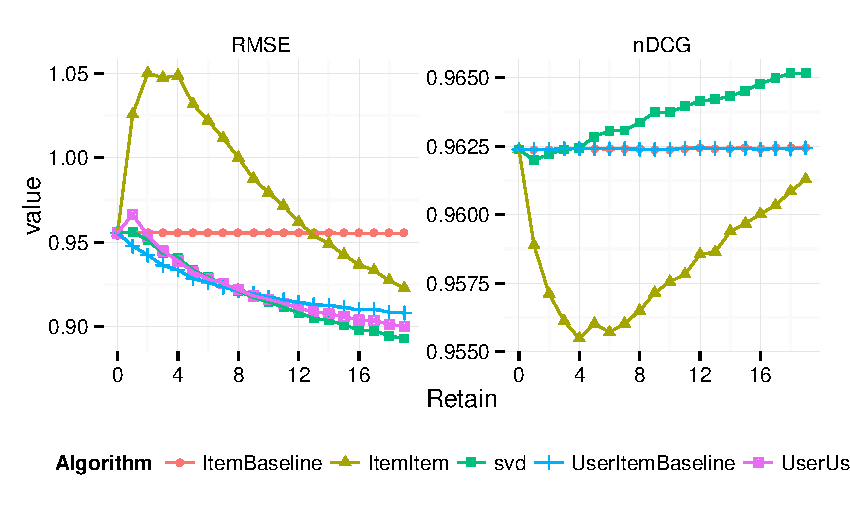
\includegraphics[width=0.666\linewidth]{../lenskit/output/ekstrandTuned20/accuracy.pdf}
  \caption{Left: RMSE, Right: nDCG}
  \label{fig:rmse}
  \label{fig:ndcg}
\end{figure*}
    % RMSE plot
    % point out error bars etc.
    % explain / interpret plot
  \paragraph{RMSE}
  Figure \ref{fig:rmse} shows how accurate our algorithms are as measured by RMSE.
  User-User, and SVD both behaved essentially as expected.
  SVD shows no improvement with only one rating, and User-User, actually appears to get worse with the first rating, but other than that, these algorithms outperform the item baseline.
  Interestingly, the User-Item baseline outperforms both algorithms until around 8 ratings, at which point both algorithms start to perform better.
  Given the size of of the differences between UserItemBaseline, UserUser, and SVD we will conclude that all three are at about the same accuracy for new users.
  That such a simple algorithm can outperform for such small values goes to show that recommending for users with very few ratings is a hard problem.
  
  Item-Item performs quite poorly for new users.
  Until we have around 14 ratings, Item-Item is less accurate than the ItemBaseline.
  In fact, for the first two ratings Item-Item appears to perform \emph{worse} as more ratings are added.
  This trend is a result of the limited coverage of the Item-Item algorithm.
  If you consider the accuracy of RMSE on only those items where it makes a personalized prediction it does show a monotonic increase in accuracy similar to the other algorithms.
  However, for small rating counts ItemItem can only predict for some percent of the item (around 60\% for users with two ratings, and around 75\% for users with four ratings).
  Because of this, many of the predictions come from the better performing UserItemBaseline.
  As we get our first few ratings, the predictions become less likely to be from the UserItemBaseline, leading to an artificial upward trend in RMSE.
  Fortunately, Item-Item seems to improve accuracy faster than the other algorithms, and therefore appears as if it will catch up.
  Unfortunately, this trend suggests that ItemItem may be unsuitable for new users.

\subsection {Recommendatin quality metrics}
  % Recommendation quality metrics
    % NDCG
  \paragraph{nDCG}
  Figure \ref{fig:ndcg} shows the algorithm's performance on the nDCG metric.
  The algorithm's behavior is very similar to the RMSE behavior.
  Both UserUser and SVD take an initial hit to accuracy at the first rating.
  This time UserUser takes much longer to recover from this and only beats the baseline after around 12 ratings.
  Again ItemItem performs quite poorly.
  This leaves SVD to perform the best, passing the baseline after about 4 ratings.
  The fact that the average item rating provides the best ranking for the first four ratings does suggest that ranking is a harder problem for recommenders to solve for new users than prediction accuracy.
  
    % MAP, precision, fallout plots 
    % explain results from MAP and precision
    % explain recall results
    % recall results, strangeness and popularity


\begin{figure*}[ht!]
  \centering
  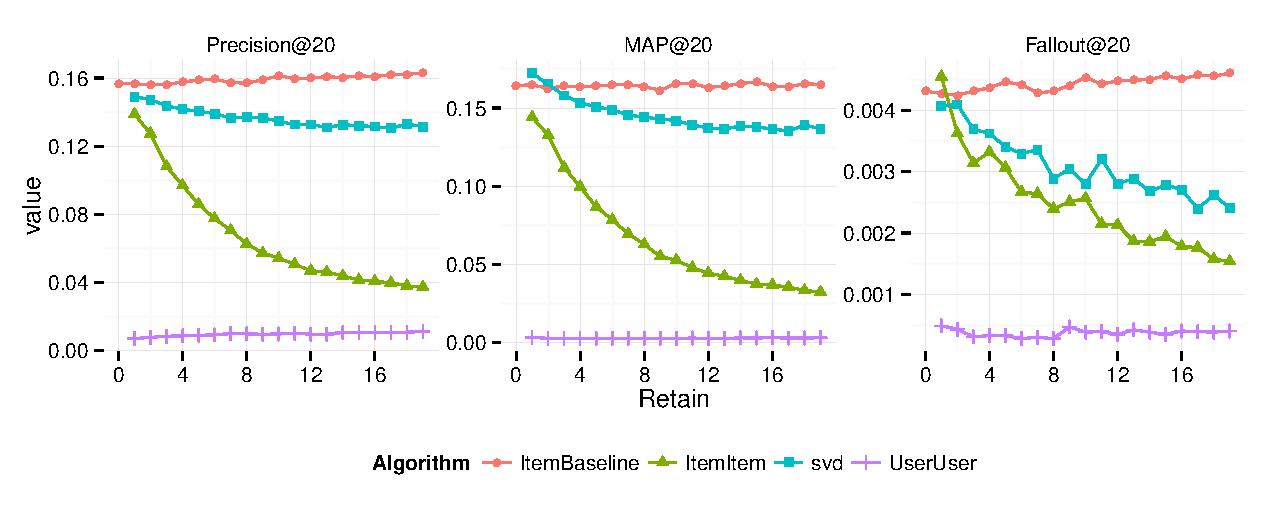
\includegraphics[width=\linewidth]{../lenskit/output/ekstrandTuned20/TopNPrecision.pdf}
  \caption{Left: Precision@20, Center: MAP@20, Right: Fallout@20}
  \label{fig:map}
\end{figure*}
\paragraph{MAP@20, Precision@20, Fallout@20}
  Figure \ref{fig:map} shows MAP@20, precision@20, and fallout@20.
  All three metrics show essentially the same trend, User-User gets the lowest score, the baseline get the highest score.
  On both MAP@20 and precision@20 svd gets a higher score than Item-Item throughout, performing almost as highly as the baseline.
  On fallout@20 Item-Item and SVD perform about as well as each other, with SVD showing a very slight lead.
  We also tested recall and mean reciprocal rank metrics, but found them to exhibit the same trend.

  This result is rather strange as MAP and precision are metrics where high scores imply better performance, whereas fallout is a metric where high scores imply poor performance.
  Therefore we would not expect to see rank equivalent behavior from these metrics.
  Unfortunately this means that these metrics contradict each other in terms of which algorithm performs the best.
  One possible reason for this is that these topN metrics are known to be biased toward recommendations that have more popular items \cite{bellogin}.
  Looking at the average popularity (figure \ref{fig:pop}) of recommended items, we see that the average popularity of the recommendations closely replicates the previous three plots.
  Therefore we will discard these metrics, and consider less biased metrics to help us analyze the quality of the recommendations.


  % TopN average rating / topn rmse
    % interpret graph and reason about what it means about quality

\begin{figure*}[ht!]
  \centering
  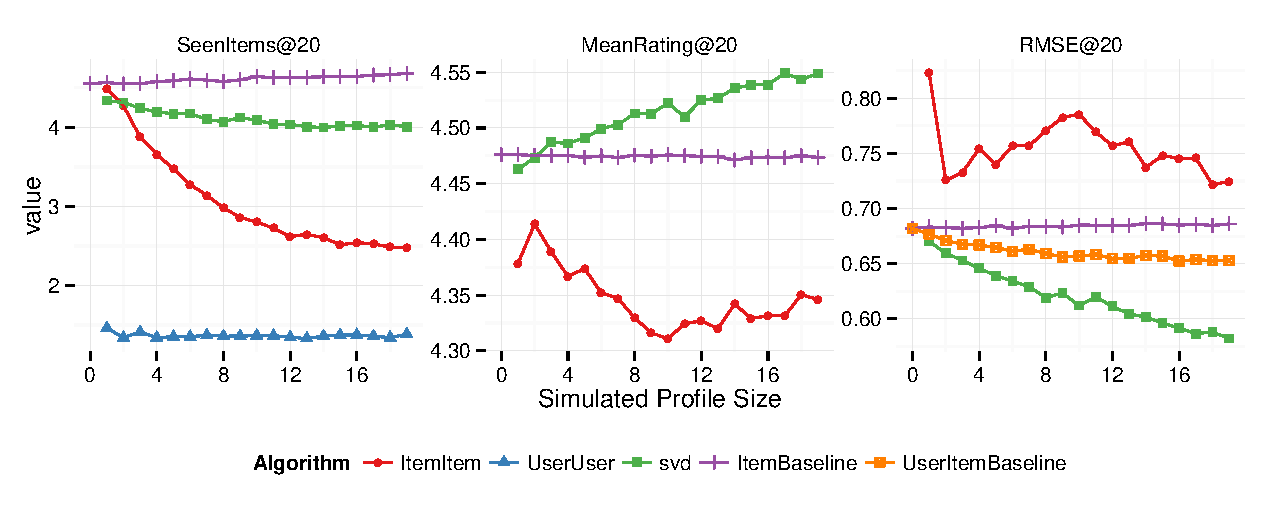
\includegraphics[width=\linewidth]{../lenskit/output/ekstrandTuned20/rmse_20.pdf}
  \caption{Left: SeenItems@20, Center: MeanRating@20, Right: RMSE@20}
  \label{fig:topN.rmse}
\end{figure*}
  \paragraph{SeenItems@20}
  The first graph in figure \ref{fig:topN.rmse} shows the average number of items in the top 20 recommendations for each algorithm that were also in the test set.
  The average number of test set items in recommendations shows a similar trend to the MAP, precision, and recall metrics, user-user getting by far the fewest seen items, and the baseline getting the most.
  As User-User gets less than one seen item on average we found that MeanRating@20 and RMSE@20 metrics were not appropriate for UserUser.
  This was observed in particular when testing our results for sensitivity to recommendation list size.
  We found that different recommendation lists led UserUser (and only UserUser) to have very different results
  Because of this issue we will not include User-User in our next evaluation and consider the next two metrics inconclusive for UserUser
  That said, we consider the small number of seen items itself a bad result for UserUser.
  Put simply, if we cannot reliably estimate if the recommendations are reasonable, how can we expect a user to do so?

  \paragraph{MeanRating@20}
  The second graph in figure \ref{fig:topN.rmse} shows the average rating for those items in the top 20 recommendations for each algorithm.
  The first thing to note about this graph is that all of these algorithms are doing a reasonable job of recommending items the user might like to watch, with all algorithms averaging above 4 stars (implying that the recommended items are, at least on average, enjoyable).
  SVD performs as expected, starting around the baseline for few ratings, and then steadily improving to be the best algorithm.
  Again, we find that Item-Item performs poorly until quite a few ratings are added, and does worse than baseline throughout.
  This is quite possibly a similar trend to the one we observed with RMSE and nDCG, where ItemItem's performance decreased as coverage increased leading to the curved performance at cold start.
    
  \paragraph{RMSE@20}
  The third graph in figure \ref{fig:topN.rmse} shows the RMSE our algorithms got on items in the top 20 recommendations for each algorithm.
  Not surprisingly, this figure shows the same trends as the last one meaning that the algorithms whose recommendations were (on average) most likable, were those whose recommendations were most accurate.
  Again, SVD performs quite well, easily bearing the UserItemBaseline after only 1 rating.
  
  Interestingly, we find that all algorithms are quite a bit more accurate on the top 20 items than they are for the general item collection.
  This is likely an edge effect, where the highest rated (5 star) items are perhaps easier to predict than other items.

\subsection{Other recommender metrics}
  % Other recommender metrics

\begin{figure*}[ht!]
  \centering
  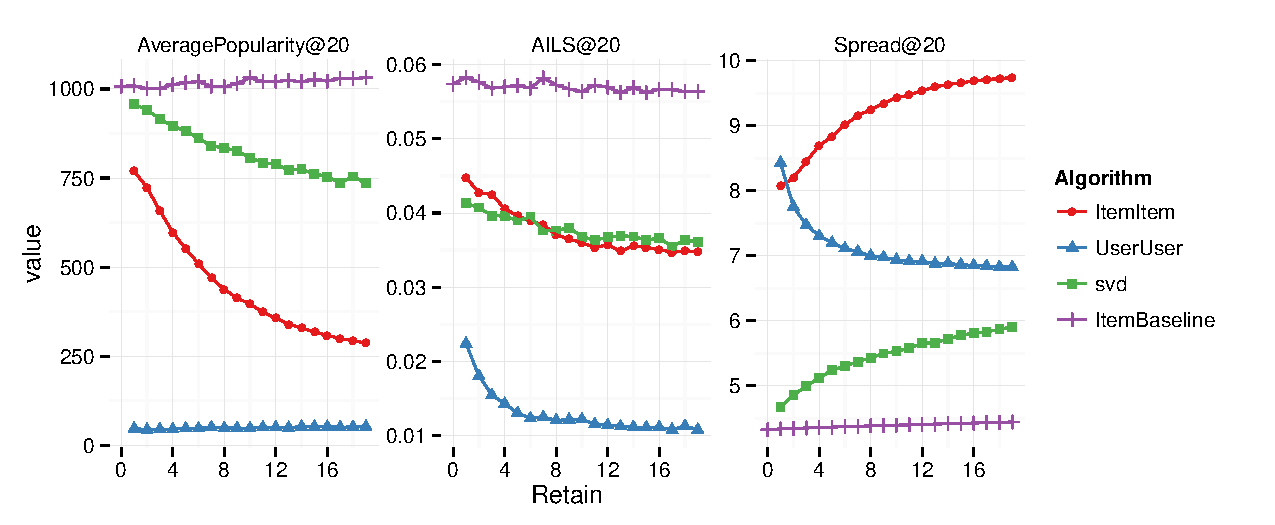
\includegraphics[width=\linewidth]{../lenskit/output/ekstrandTuned20/popdiv.pdf}
  \caption{Left:averagePopularity@20, Center AILS@20, Right Spread@20}
  \label{fig:pop}
\end{figure*}

  \paragraph{AveragePopularity@20}
    % popularity graph
  The first graph in figure \ref{fig:pop} shows the average popularity of recommended items by each algorithm.
  As expected the baseline algorithms make the most popular recommendations, followed by SVD, ItemItem, and then UserUser in a distant last.
  Unfortunately, we don't know of any guideline for understanding how popular users desire their recommendations to be.
  That said, we expect that users will feel the baseline's popularity (around 1000) is too high, and User-User's popularity (around 50) is too low.
  SVD and Item-Item both seem to perform well, with SVD generating more popular recommendations than Item-Item.
  SVD and ItemItem both show a trend of decreasing popularity as more ratings are retained, suggesting that these algorithms will make more nuanced, less popular recommendations for users they know more about.
  Interestingly, these algorithms each appear to be converging to their own separate level of popularity, which suggests that this ordering may be independent of number of items retained.

    % diversity plot
  \paragraph{AILS@20}
  The second graph in \ref{fig:pop} shows a similar trend to the popularity trend with the baseline algorithms producing the least diverse list of recommendations and User-User providing by far the most diverse list of recommendations.
  Unlike popularity, SVD and ItemItem seem to perform equivalently in diversity.
  In terms of diversity we see that all three collaborative filtering algorithms show a trend of increasing diversity (decreasing  inter-list similarity) as more ratings are retained.

  % spread plot
  \paragraph{Spread@20}
  The third graph in \ref{fig:spread} shows the spread of the recommendations from each algorithm.
  Because this metric can only be computed over a group of people, confidence intervals over the per-user average are not provided, instead the specific spread values computed in each five folds are shown as points, with lines connecting the average values.
  As expected the baseline performs worst on spread, as it recommends the same items to each user, unless the user has already rated one of these items.
  SVD performs mildly better than the baseline, and shows definite improvement as more ratings are added.
  UserUser and ItemItem start at around the same value as each other, however, after only two ratings they have crossed, as ItemItem quickly increases to have the highest spread of all the algorithms, and UserUser quickly decreases into second place.
  Interestingly, only UserUser shows a trend to have less spread ratings as it learns more about the user, ItemItem and SVD both show the expected trend of increasing Spread as they learn more.
  This could be some form of a regression towards the mean, where as it learns more about users its recommendations become less personalized to the users individual quirks.
  More research will be needed to understand this trend.
  
\section{Conclusions}
  % summary of results in a big old table.
    % the accuracy of svd and user-user both seemed good. item-item seemed to have trouble especially with very new users.
    % svd did quite well on our traditional topN metrics, item-item did OK, and user-user did bad., but there are flaws with these metrics.
    % on our topN RMSE item-item (again) seemed to have issues, and user-user did quite well, but the low hit rate is troubleing. 
    % again svd seems the winner here.
    % on our fluffy metrics item-item and svd seemed to do well. I might argue that item-item seemed to do better (spread, and higher throughout).
    % user-user seemed to do poor

  % what this means
    % user-user seems to be able to give accurate predictions, but seems to focus on overly obscure items in recommendation.
    % item-item seems to give not-bad recommendations, but its predictions have issues
    % based only on these results svd seems to be the best performer and is our recommendation to new systems.
    
  \begin{table}[ht!]
    \centering
    \begin{tabular}{|p{4.5em}|p{4.5em}|p{7.5em}|p{4.5em}|}
      \hline
      Algorithm & Perdiction accuracy & Recommendation quality      & Other properties \\\hline
      ItemItem  & Poor                & Poor                        & Good             \\\hline
      SVD       & Good                & Good                        & Good             \\\hline
      UserUser  & Good                & Inconclusive                & Poor             \\\hline
    \end{tabular}
    \caption{Summary of algorithm quality for new users}
    \label{tbl:results}
  \end{table}

  The high level results of our evaluation are summarized in table \ref{tbl:results}
  Overall we see that SVD seems to be the best performing algorithm for cold start use.
  SVD was the only algorithm that consistently outperformed the baseline algorithms on prediction and recommendation tasks.
  ItemItem had arguably better results on the average popularity and spread metrics, indicating that it was able to find more novel items, and make a larger range of recommendations to users.
  Unfortunately, Item-Item also performed quite poorly at both prediction and recommendation, which may make it less suitable for new users.

  UserUser performed quite well are prediction, but tended to favor unpopular items in its recommendations.
  While some novelty is good, we believe that UserUser goes too far into the obscure movies in its recommendations, and therefore does not make good recommendations.
  Therefore we believe that UserUser is not well suited to new users if its recommendations are going to be used.
  Exploring corrections for this issue is left as future work.

  % other takeaways
    % regularization
  This analysis suggests that, at least for new users, system designers use algorithms from the SVD family.
  We belive that it is the regularization built into these algorithm that give them good performance.
  UserUser and ItemItem algorithms have no built in method for damping their predictions towards the mean when they don't have much data.
  The regularization in the cost function of the SVD model makes it so its predictions will gradually shift away from the baseline predictions as more relevant ratings are added.
  The downside of this, however, could be the higher popularity and lower spread seen by the SVD algorithm.
  The same regularization that helps avoid making mistakes due to too little data, may also prevents the algorithm from taking occasional risks on more obscure movies.

    % if you use a switching recommender, this methodology can help you choose when to switch.
    % non-traditional metrics can tell you more about what is going on, these seem to be more properties of the class of algo than of the data, so its worth looking at these when choosing algorithms, to find one with properties that are good for your task.
  One interesting result of our analysis is that at very small numbers of ratings the UserItemBaseline seems to be our strongest algorithm, both in terms of accuracy (as measured by RMSE), and in terms of recommendation quality (as measured by MeanRating@20).
  This suggests a recommendation strategy for live systems.
  Instead of recommending from one recommender right away, a system could provide baseline predictions and recommendations until the user has enough ratings and then switching to a better recommender.
  For recommenders like this our methodology provides a way to find the correct number of ratings at which to switch algorithms.


  % limitations and opprotunities
    % dataset limitations
      % only one domain
      % no quitters in our dataset

  One of the major limitations of our work is that we only evaluated one dataset.
  Future work should replicate our experiment on other datasets from different recommender domains.
  By doing this we will find out which of our results are true properties of the algorithms, and which results are instead related to properties of our dataset.

  One important property that needs to be considered is that our dataset only contained users that naturally used the system enough to collect 20 ratings.
  Unfortunately, this means that we do not know if there are differences between users who do and do not survive in the system.
  This is a limitation of our methodology, to maintain a constant test set throughout the evaluation we are not able to evaluate users who have less ratings than the maximum amount we wish to study.
  More work needs to be done to understand users who only ever make one or two ratings to understand why they leave, and how they differ from other users of our systems.

  Finally, we feel that much more work should be done using this methodology to explore different algorithms.
  There are many algorithms beyond the three e evaluated.
  Some of these algorithms are designed specifically for cold start.
  Others are designed to leverage extra, non-rating information to improve quality.
  Work should be done to understand the differences between these algorithms, and what effect extra information has on the recommendation process.
  Using our methodology we might be able to come up with an understanding of the value that extra information about the user has on recommendation, and to compare it the value of extra ratings for new users.
    % algorithm limitations
      % only covered three common families,
      % different algos tuned specifically for cold start.
      % algos that use extra data about users or about items.
    % cite the comparison work at CHI.

  % despite the limitations we were able to show differences between algorithms in a cold start situation.

\section{Acknowledgements}
 TODO:

\bibliographystyle{abbrv}
\bibliography{resources}  % sigproc.bib is the name of the Bibliography in this case

\end{document}
